\documentclass[]{commands}
\usepackage{afterpage}
\usepackage{hyperref}
\usepackage{color}
\usepackage{xcolor}
\PassOptionsToPackage{cmyk}{xcolor}
\usepackage{fontspec}
\usepackage{fontawesome}
\usepackage{marvosym}
\usepackage{textcomp}
\usepackage{float} % to position signature
\usepackage{adjustbox}
\usepackage{calc}
\usepackage{enumitem} % to customize indent of bullet points via \itemize
\usepackage{metalogo}
\usepackage{dtklogos}
\usepackage[utf8]{inputenc}	
\usepackage{tikz}
\usetikzlibrary{mindmap,shadows,positioning}
\hypersetup{
    pdftitle={},
    pdfauthor={},
    pdfsubject={},
    pdfkeywords={},
    colorlinks=false,           % no lik border color
    allbordercolors=white       % white border color for all
}

% \addbibresource{bibliography.bib}
\RequirePackage{xcolor}
\definecolor{lightgray}{HTML}{777788}
\definecolor{centergray}{HTML}{B9B9C9}
% you can change ipsgreen to any color you like, but you´ll also have to change it in the reccius-cv-experiment.cls file
\definecolor{ipsgreen}{HTML}{3B6746}

% NAME AND TAGLINE
\begin{document}
\header{Carlos}{ Franzreb}{}
      
\vspace{0.3cm}   
\color{lightgray}\noindent\makebox[\textwidth]{\rule{\paperwidth-0.4cm}{2.5pt}}
% In the aside, each new line forces a line break

% CONTACT
\begin{info}
    \begin{flushleft}
    \small{20. May 1997}\hfill{\faCalendar}\\
    
    \vspace{1mm}

    \small{Berlin, Germany}\hfill{\faMapMarker}\\
    
    \vspace{1mm}
    
    {\small +49 1575 2836912}\hfill{\Mobilefone}\\

    \vspace{.8mm}
    
    \href{mailto:carlosfranzreb@gmail.com}{\small{carlosfranzreb@gmail.com}\hfill{\Large\Letter}\hspace{0.6mm}{\small \faMousePointer}}\\
    
    \href{https://github.com/carlosfranzreb}{\small{carlosfranzreb}\hfill{\Large\faGithub}\hspace{0.6mm}{\small \faMousePointer}}\\
    
    \end{flushleft}
\end{info}

% SIDE BAR
\begin{aside}
    ~

% PICTURE
\vspace{-3.5cm}
\begin{figure}[ht]
	\hspace{0.3cm}
	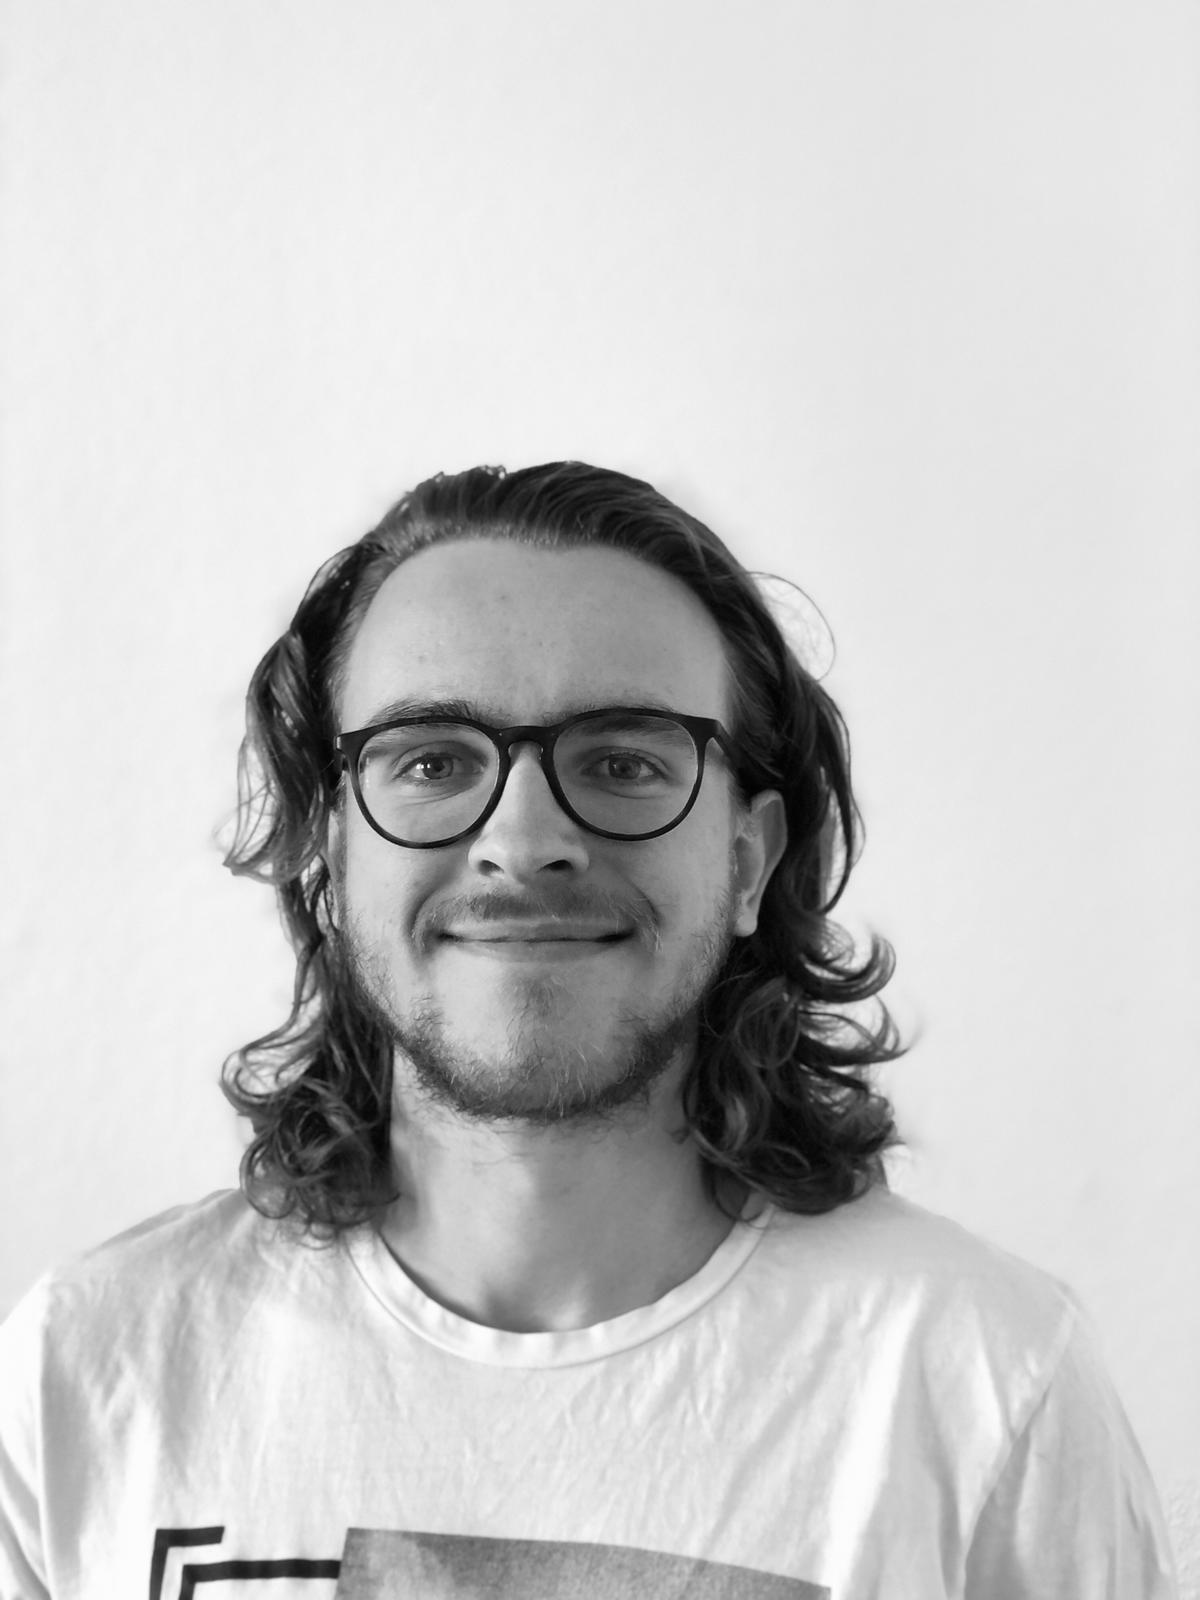
\includegraphics[width=.71\linewidth]{img/portrait.jpg}
\end{figure}

% INTERESTS
\vspace{3.5mm}
\section{Interests}
\vspace{3.5mm}

I am interested in algorithms, especially those that learn from data. I find the whole process appealing, from deciding on how to store the data to designing the visualization of the results.


% LANGUAGES
\vspace{3.5mm}
\section{Languages}
\vspace{3.5mm}

\textbf{German}\hfill

\includegraphics[scale=0.11]{img/IPSGreenDots.png}

\includegraphics[scale=0.11]{img/IPSGreenDots.png}

\includegraphics[scale=0.11]{img/IPSGreenDots.png}

\includegraphics[scale=0.11]{img/IPSGreenDots.png}

\includegraphics[scale=0.11]{img/IPSGreenDots.png}

\textbf{Spanish}\hfill

\includegraphics[scale=0.11]{img/IPSGreenDots.png}

\includegraphics[scale=0.11]{img/IPSGreenDots.png}

\includegraphics[scale=0.11]{img/IPSGreenDots.png}

\includegraphics[scale=0.11]{img/IPSGreenDots.png}

\includegraphics[scale=0.11]{img/IPSGreenDots.png}

\textbf{English}\hfill

\includegraphics[scale=0.11]{img/IPSGreenDots.png}

\includegraphics[scale=0.11]{img/IPSGreenDots.png}

\includegraphics[scale=0.11]{img/IPSGreenDots.png}

\includegraphics[scale=0.11]{img/IPSGreenDots.png}

\includegraphics[scale=0.11]{img/IPSGreenDots.png}

% SKILLS
\vspace{3.5mm}
\section{Skills}
\vspace{3.5mm}

\textbf{Python}\hfill

\includegraphics[scale=0.11]{img/IPSGreenDots.png}

\includegraphics[scale=0.11]{img/IPSGreenDots.png}

\includegraphics[scale=0.11]{img/IPSGreenDots.png}

\includegraphics[scale=0.11]{img/IPSGreenDots.png}

\includegraphics[scale=0.11]{img/WhiteDots.png}

\textbf{Machine learning}\hfill

\includegraphics[scale=0.11]{img/IPSGreenDots.png}

\includegraphics[scale=0.11]{img/IPSGreenDots.png}

\includegraphics[scale=0.11]{img/IPSGreenDots.png}

\includegraphics[scale=0.11]{img/IPSGreenDots.png}

\includegraphics[scale=0.11]{img/WhiteDots.png}

\textbf{Databases}\hfill

\includegraphics[scale=0.11]{img/IPSGreenDots.png}

\includegraphics[scale=0.11]{img/IPSGreenDots.png}

\includegraphics[scale=0.11]{img/IPSGreenDots.png}

\includegraphics[scale=0.11]{img/IPSGreenDots.png}

\includegraphics[scale=0.11]{img/WhiteDots.png}

\textbf{Java}\hfill

\includegraphics[scale=0.11]{img/IPSGreenDots.png}

\includegraphics[scale=0.11]{img/IPSGreenDots.png}

\includegraphics[scale=0.11]{img/IPSGreenDots.png}

\includegraphics[scale=0.11]{img/WhiteDots.png}

\includegraphics[scale=0.11]{img/WhiteDots.png}

\textbf{JS, HTML, CSS}\hfill

\includegraphics[scale=0.11]{img/IPSGreenDots.png}

\includegraphics[scale=0.11]{img/IPSGreenDots.png}

\includegraphics[scale=0.11]{img/IPSGreenDots.png}

\includegraphics[scale=0.11]{img/WhiteDots.png}

\includegraphics[scale=0.11]{img/WhiteDots.png}

% Other interests
\vspace{3.5mm}
\section{Other interests}
\vspace{3.5mm}

\faBook \hspace{3mm} \textbf{Reading}

\faPaintBrush \hspace{3mm} \textbf{Art}

\faTrophy \hspace{3mm} \textbf{Chess}

\faSigning \hspace{3mm} \textbf{Climbing}

\faBattery \hspace{3mm} \textbf{Running}

\end{aside}

\newcommand{\eduspace}{\vspace*{0.85mm}}
\newcommand{\eduspaceII}{\vspace*{0.8mm}}
\newcommand{\jobspace}{\vspace*{-4.2mm}}

% EXPERIENCE
\section{Experience}
\begin{entrylist}
  \entry
    {June 2020 - now}
    {Research assistant | }
    { \href{https://www.fokus.fraunhofer.de/}{\small Fraunhofer FOKUS \faMousePointer}}
    {\normalsize\textbf{\color{ipsgreen}\faMapMarker\space Berlin}}
    {\jobspace
    \begin{itemize}[leftmargin=*, itemsep = 0.1em]
        \item Interdisciplinary research with sociologists on digitalization and science.
        \item Developed a data harvester with Vert.x (asynchronous programming).
        \item Research on knowledge graph embeddings and subject indexing.
        \item Retrieved and visualized tweets with D3.js to analyse the spread of \\ 
            misinformation for a paper which has been submitted for review.\\
    \end{itemize}}

  \entry
    {May 2019 - May 2020}
    {Business developer | }
    { \href{https://www.365farmnet.com/en/}{\small 365FarmNet \faMousePointer}}
    {\normalsize\textbf{\color{ipsgreen}\faMapMarker\space Berlin}}
    {\jobspace
    \begin{itemize}[leftmargin=*, itemsep = 0.1em]
        \item Visualized the journey of the users in the company's software.
        \item Developed a software tool that predicted the impact of a new \\
            feature based on the marketing personas. \\
    \end{itemize}}
    
  \entry
    {Sep. 2018 - Dec. 2018}
    {Intern | }
    { \href{https://www.dezem.de/en/}{\small deZem \faMousePointer}}
    {\normalsize\textbf{\color{ipsgreen}\faMapMarker\space Berlin}}
    {\jobspace
    \begin{itemize}[leftmargin=*, itemsep = 0.1em]
        \item Developed software to automate processes of the marketing team.
        \item Translated software manuals and assisted users with the software. \\
    \end{itemize}}
    
  \entry
    {Sep. 2017 - Oct. 2017}
    {Intern | }
    { \href{https://thecloud.group/}{\small The Cloud Group \faMousePointer}}
    {\normalsize\textbf{\color{ipsgreen}\faMapMarker\space Madrid}}
    {\jobspace
    \begin{itemize}[leftmargin=*, itemsep = 0.1em]
        \item Designed databases with SQL for various software tools. 
        \item Full-stack development of software with PHP, JQuery, HTML5 and CSS3. \\
    \end{itemize}}
    
  \entry
    {Sep. 2016 - Oct. 2016}
    {Intern | }
    { \href{https://www.siemens.com/global/en.html}{\small Siemens \faMousePointer}}
    {\normalsize\textbf{\color{ipsgreen}\faMapMarker\space Berlin}}
    {\jobspace
    \begin{itemize}[leftmargin=*, itemsep = 0.1em]
        \item Worked in a factory of the energy management division. \\
    \end{itemize}}
    
  \entry
    {Sep. 2013 - May 2015}
    {Basketball coach | }
    { \href{https://colegiosanpatriciomadrid.com/en/our-campuses/school-el-soto/extra-curricular-activities/}{\small Colegio San Patricio \faMousePointer}}
    {\normalsize\textbf{\color{ipsgreen}\faMapMarker\space Madrid}}
    {\jobspace
    \begin{itemize}[leftmargin=*, itemsep = 0.1em]
        \item Assistant coach during my last two high school years. \\
    \end{itemize}}
    
\end{entrylist}

% EDUCATION
\section{Education}
\begin{entrylist}
 
   \entry
    {Oct. 2019 - Oct. 2021}
    {MS Computer Science | }
    { \href{https://www.tu.berlin/en/}{\small TU Berlin \faMousePointer}}
    {}
    {\jobspace
    \begin{itemize}[leftmargin=*, itemsep = 0.1em]
        \item Focus on cognitive systems.
        \item Project: developed a small relational database with Java.
        \item Project: built an LSTM network for protein structure prediction in PyTorch.
        \item Thesis: Subject indexing for institutional repositories.\\
    \end{itemize}}
    
  \entry
    {Oct. 2015 - Oct. 2019}
    {BS Computational Engineering Science | }
    { \href{https://www.tu.berlin/en/}{\small TU Berlin \faMousePointer}}
    {}
    {\jobspace
    \begin{itemize}[leftmargin=*, itemsep = 0.1em]
        \item Thesis: Evaluating FaaS as a data import agent.\\
    \end{itemize}}

  \entry
    {Sep. 2009 - May 2015}
    {High School | }
    { \href{https://colegiosanpatriciomadrid.com/en}{\small Colegio San Patricio \faMousePointer}}    {\normalsize\textbf{\color{ipsgreen}\faMapMarker\space Madrid}}
    {}
    
  \entry
    {Aug. 2012 - May 2013}
    {Year abroad | }
    { \href{https://www.mercersburg.edu/}{\small Mercersburg Academy \faMousePointer}}    {\normalsize\textbf{\color{ipsgreen}\faMapMarker\space Pennsylvania, USA}}
    {}
\end{entrylist}

% PROJECTS
\section{Other projects}
\begin{entrylist}
 
   \entry
    {Dec. 2019 - now}
    {Cooking blog | }
    {\href{https://www.saludypimienta.com/}{\small Salud y Pimienta \faMousePointer}}
    {}
    {\jobspace
    \begin{itemize}[leftmargin=*, itemsep = 0.1em]
        \item A website for my mother's recipes developed with Flask (Python).\\
    \end{itemize}}
    
   \entry
    {Jan. 2017 - May 2017}
    {Employee scheduling software}
    {}
    {}
    {\jobspace
    \begin{itemize}[leftmargin=*, itemsep = 0.1em]
        \item A scheduling software developed with PHP and AJAX for a small company.\\
    \end{itemize}}
    \vspace{-4mm}
\end{entrylist}

\end{document}
